%%
%% This is file `mcmthesis-demo.tex',
%% generated with the docstrip utility.
%%
%% The original source files were:
%%
%% mcmthesis.dtx  (with options: `demo')
%%
%% -----------------------------------
%%
%% This is a generated file.
%%
%% Copyright (C)
%%     2010 -- 2015 by Zhaoli Wang
%%     2014 -- 2016 by Liam Huang
%%
%% This work may be distributed and/or modified under the
%% conditions of the LaTeX Project Public License, either version 1.3
%% of this license or (at your option) any later version.
%% The latest version of this license is in
%%   http://www.latex-project.org/lppl.txt
%% and version 1.3 or later is part of all distributions of LaTeX
%% version 2005/12/01 or later.
%%
%% This work has the LPPL maintenance status `maintained'.
%%
%% The Current Maintainer of this work is Liam Huang.
%%
\documentclass{mcmthesis}
\mcmsetup{CTeX = false,   % 使用 CTeX 套装时,设置为 true
        tcn = 2014906, problem = A,
        sheet = true, titleinsheet = true, keywordsinsheet = true,
        titlepage = true}
\usepackage{palatino}
\usepackage{mwe}
\usepackage{graphicx}
\usepackage{subcaption}
\usepackage{float}
\usepackage{multirow}
\usepackage{indentfirst}
\usepackage{gensymb}
\usepackage[ruled,lined,commentsnumbered]{algorithm2e}
\usepackage{geometry}

%% ADDED
\usepackage{mathtools}
\usepackage{setspace}



\begin{document}
\linespread{0.6} %%行间距
\setlength{\parskip}{0.5\baselineskip} %%段间距

\title{Novel Coronavirus Pneumonia: Aloha and to Say Aloha}

\date{\today}
	\begin{abstract}
\hspace{1.2em}
	Begin Abstract...
		\begin{keywords}
			Begin Keywords...
		\end{keywords}
	\end{abstract}


\maketitle

\tableofcontents

\newpage


\section{Introduction}	\label{S1}

\subsection{Problem Background}
	The ocean is covering approximately 1.3 billion cubic kilometers on Earth, which is the equivalent of 97 percent of total water. Playing a vital role in oxygen producing, carbon sequestering and food providing for billions of people, the ocean's abilities are being eroded by plenty of stressors. \par
	Since the 1950s, the oceans hava absorbed more than 93 percent of all the heat that produced by human, which is beginning to show its drawbacks at a price. Marine organisms, as an import part in the ocean, can be affected when there are changes in their natural habitat as well as changes in ocean chemistry. As a primary producer of the food chain in the ocean, phytoplankton, a kind of marine plants, is facing a slowly decrease if the water becomes warmer, which results in the reduction of the amount of nutrients in the ocean. The scarcity of nutrients will limit the growth of marine organisms in the food chain. In addition, temperature plays an important role in controlling biological rhythm of marine plants and animals involving birth, growth, feeding, production and death. The changes in ocean temperature will cause a disruption of biological rhythm making marine organisms become vulnerable to illness. Moreover, sequence lowering of the pH of seawater is unfavorable to the hatching of eggs and the growth of fry of some sea fish.\par
	The anticipated increase in ocean temperature is predicted to stimulate the migration of marine organisms based on their temperature tolerance, with heat-tolerant species expanding their range northward and those less tolerant species retreating. Just as the lobster of Maine, USA, thousands of aquatic species is forced to migrating north to find a better habitat. As an impact, relative companies need to move their base to survive. \par
	

\subsection{Our Work}
	

	The major logic flow is depicted as follows, in Figure \ref{fig:flow}:
	
	\begin{figure}[H]
    \centering
    \includegraphics[width=1\textwidth]{plots/flow_V1.jpg} %%% \textwidth 可以改图片大小
    \caption{Major Logic Flow of our Model - ALOHA}
    \label{fig:flow}
    \end{figure}
    %% Flow Chart %%%


\section{Assumptions and Justifications}\label{S2}
    We make some general assumptions to simplify our model. We will list all of the assumptions together with corresponding justification below:
\begin{enumerate}[1)]
	\item {\bfseries All of human beings are susceptible to NCP.} NCP was recently discovered and has gene specificity, which make it difficult to be immunized by the body. Thus, we can infer that human beings are susceptible to this virus without previous contact.
	\item {\bfseries People will not get susceptible to secondary infection of NCP.} Depending on the nature of the body's immune system, after recovery most people will have better immune reaction to virus. We ignore the possibility of secondary infection to simplify our model.
	\item {\bfseries Assume that incubation period to different individuals are the same.} Since incubation period of different host individual is different and also hard to predict, we assume that incubation periods are the same.
	\item {\bfseries NCP will only complete the process of human-to-human transmission via close contact such as talking face-to-face.} We simplify our model here since people suffer a rather low  level of risk if they do not have close contact with the infected when it comes to NCP.
	\item {\bfseries The number of infected people around the world is almost the number of infected people in China}. Although countries except China accounts for 71.57\% of the world population \small{(till August 28th, 2019, by United Nations \cite{pop_un})}, only less than  0.77\%of confirmed cases occurred outside China \small{(till February 3rd, 2020, by various organizations \cite{cov_who}\cite{cov_tencent}\cite{cov-jhu}\cite{cov-cdc}; with detailed information listed in Appendix)}. Meanwhile, after NCP was discovered in China, all the other countries took immediate action against the spread. Therefore, what deserves our attention is more the circumstances in China.
\end{enumerate}


\section{Notations and Definitions}\label{S3}
    For convenience, we define a series of notations for mathematical usage, which are listed in Table \ref{notation} to describe our model.
\begin{table}[H]\large
    \centering
    \caption{Notations mentioned in this paper}
    \label{notation}
    \begin{tabular}{c c}
\toprule[2pt]
        Symbol & Definition\\
\hline
    $S(t)$ & Number of susceptible person at time t\\
    $E(t)$ & Number of enfective person at time t\\
    $I(t)$ & Number of infectious person at time t\\
    $R(t)$ & Number of removed person at time t\\
    $t$ & Time\\
    $N$ & Gross population in this model\\
    $\alpha$ & Morbidity of NCP\\
    $\beta$ & Infection rate\\
    $\gamma$ & Removal rate\\
    $d$ & Mortality of NCP\\
    $h$ & Recovery rate of NCP\\
    $k$ & Average number of people exposed to infections every day \\
    $b$ & Probability of infection by contact\\
    $R_0$ & Basic reproduction number\\
    $m_i$ & Affecting parameters of $ith$ measure by government \\
    $ND$ & Number of death\\
    $NR$ & Number of recovery\\
    $NSP$ & Number of suspected people\\
    $NDP$ & Number of diagnosed people\\
\bottomrule[2pt]
    \end{tabular}
\end{table}



\section{Model Analysis} \label{S4}
		In this section, we present the \emph{Gray Forecasting} method to simulate the change of the average sea surface temperature of a region on the ocean. Also, we use \emph{Differential Equation} to introduce the influence of global warming to the temperature. The framework of the model is shown in Figure 1. Referencing the temperature data onto recent years, we calculate the factors of our model using Gray Forecasting, which can identify the degree of variation in development trends among system factors. After conducting the solution by Gray Forecasting, we additional add the global warming factor of the heavier of carbon emission. Finally, we analyze the immigration of these two fish species as well as the most likely location for these two fish species over the next 50 years.
	% ADD Flow Chart of Model 1

\subsection{Sea Surface Temperature Forecasting Model}\label{S4s1}
	The temperature on the ocean always gets affected by a huge number of factors, including solar radiation, ocean currents, carbon emission, Nino phenomenon, etc. To avoid the complex analysis and simplify the problem, we use a gray forecasting model to calculate the correlation degree of factors. Besides, the acceleration of global warming, extra differential equations are needed as correction of our model.

\subsubsection{SST Based on Gray Forecasting}\label{S4ss1}
	We first denote the symbols and terms used in this part.
\begin{table}[H]\large
    \centering
    \caption{Symbols and Terms}
    \label{symbol}
    \begin{tabular}{c c}
\toprule[2pt]
        Symbol & Definition\\
\hline
    $AGO$ & Accumulated Generating Operation\\
    $GM(1,1)$ & Gray Model\\
    $IAGO$ & Inverse Accumulated Generating Operation\\
    $...$ & ...\\
\bottomrule[2pt]
    \end{tabular}
\end{table}
	According to the already existing SST data, we choose from 2006.1 as the first month to 2020.1.\par
	Assuming that the SST in the original k-th month is $x^{(0)}(k)$, set the original data as follows: $ x^{(0)} = x^{(0)}(1), x^{(0)}(2), ..., x^{(0)}(n)$\par
	We denote
\begin{equation*}
	x^{(1)}(k) =  \sum_{i=1}^kx^{(0)}(i) \qquad  ,where k = 1, 2, ..., n
\end{equation*}\par
	Then, we calculate the class ratio $\lambda{k}$
\begin{equation*}
	\lambda(k) =  \frac{x^{(0)}(k-1)}{x^{(0)}(k)}
\end{equation*}\par
	Due to all $\lambda k \in \big[0.982, 1.0098\big]$, we can reach a fatisfying model using GM(1,1).
	By $AGO$, 
\begin{equation*}
	x^{(1)}(k) =  \sum_{i=1}^kx^{(0)}(i) \qquad  ,where k = 1, 2, ..., n
\end{equation*}\par
	Take differential, i.e.
\begin{equation*}
	d(k) = x^{(0)}(k) = x^{(1)}(k) - x^{(1)}(k-1)
\end{equation*}\par
	Denote $z^{(1)}(k)$ as the adjacent value generated sequence, i.e.
\begin{equation*}
	z^{(1)}(k) = \alpha x^{(1)}(k) + (1-\alpha)x^{(1)}(k-1)
\end{equation*}\par
	So, we get the model as
\begin{equation*}
	d(k) = \alpha z^{(1)}(k) = b
\end{equation*}\par
	We then construct Data Matrix $B$ and Data Vector $Y$
\begin{equation}
	B =  \left[ \begin{matrix}
						-\frac{1}{2}(x^{(1)}(1)+x^{(1)}(2))  & 1 \\
						-\frac{1}{2}(x^{(1)}(2)+x^{(1)}(3))  & 1 \\
										...									& ... \\
						-\frac{1}{2}(x^{(1)}(k)+x^{(1)}(k+1))  & 1 \\
\end{matrix}\right],
	Y =  \left[ \begin{matrix}
						x^{(0)}(2)\\
						x^{(0)}(3)\\
							...    \\
						x^{(0)}(k)\\
\end{matrix}\right]
\end{equation}\par
\begin{equation*} 
	\hat{\mu} = (a, b)^{T} = (B^{T}B)^{-1}B^{T}Y = ???
\end{equation*}\par
\begin{equation*}
	\frac{dx^{(1)}}{dt} + ?? x^{(1)} = ??
\end{equation*}\par
	Solution is, 
\begin{equation*}
	x^{(1)}(k+1) = (x^{(1)}(k) - \frac{b}{a})e^{-ak} + \frac{b}{a} = ???
\end{equation*}
	Until now, we get the forecasting value of future sea surface temperature.\par
	
\subsubsection{Influence of Global Warming}\label{S4ss2}
	Equation \ref{set1} shows the mathemetical fundation of the influence of global warming. The parameters are defined as follows:

\begin{itemize}
	\item $\rho$ indicate the density of the ocean. Since there are only delicate distinction between different region, we let $\rho$ approximately equal to 1. 
	\item \emph{h} shows the mixed layer depth, which we take
		\begin{equation*}
		\emph{h}  = 70m
		\end {equation*}
	\item $C_p$ shows the specific heat of a part of ocean, which is defined as 
		\begin{equation*}
		Cp\quad za\quad qiu\quad de ???
		\end {equation*}
	\item $\gamma$ is a parameter defined in terms of the fraction of land. We assume $\gamma \in \big[0.72,0.75\big]$ 
	\item $\lambda$ the climatic feedback factor, which is defined as 
		\begin{equation*}
		\lambda = 3.58
		\end {equation*}
	\item  $\delta F$ express the flux lost from the mixed layer, which is ignored in our model. 
		
	\item $\delta Q$ shows the net surface flux, which is defined as
		\begin{equation*}
		\delta Q = 34.6534 \times 10^{-4}te^{8.686\times 10^{-3}t}
		\end {equation*}
	\item \emph{t} indicates the number of the year, such as 2018, 2019, etc.
\end{itemize}
\begin{equation*}\label{set1}
\gamma\rho C_{p} h\frac{d\delta t}{dt} = \delta Q - \lambda\delta T - \delta F
\end{equation*}
\par

\subsection{Fish Immigration}\ref{S4s3}
	


\section{title}\label{S5}

\subsection{Background Illustration}
   
    
\subsection{subsection1}\label{S5s1}
    

\subsection{subsection2}\label{S5s2}
	
 
\section{S6}\label{S6}
   
	
\subsection{Simulation Results}
    


\section{Model Analysis}\label{S7}

\subsection{Sensitivity Analysis}


\subsection{Strengths and Weaknesses}
\subsubsection{Strengths}
\begin{itemize}
	\item Our model achieves a good simulation in fitting the current infections.
	\item Our model takes into account the effects of the change of pedestrian flow during the Spring Festival travel rush as well as virus mutations
	\item The model is a well-organized epidemic model which can be widely applied to other virus disease.
\end{itemize}
\subsubsection{Weaknesses}
\begin{itemize}
	\item The prediction simulation result can't be verified due to the unknown data in future.  
	\item A large number of assumptions reduce the accuracy of the model’s simulation results.
\end{itemize}


\section{Conclusion}\label{S8}


\newpage


\bibliographystyle{IEEEtran}
\bibliography{newrefs}

\section*{Brief Assessment Report}\label{S9}

\newpage

\begin{appendices}

\section{Solve and Plot Ordinary Differential Equation Systems}
\lstinputlisting[language=Python]{ODES.py}

\end{appendices}


\newpage


% \section{Figures}

% %%  单图片模型(不要复制这句话)
% 	\begin{figure}[H]
%     \centering
%     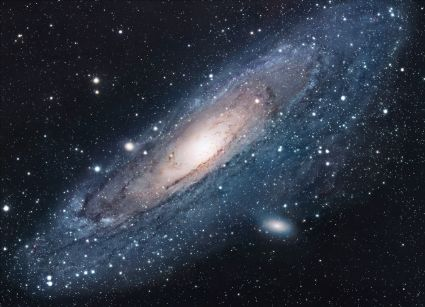
\includegraphics[width=0.7\textwidth]{universe.jpg}%%% \textwidth 可以改图片大小
%     \caption{biao ti ?}
%     \label{Fig_1}
%     \end{figure}
%     %%% 需要的话,请在这里写图片说明,否则不要复制 %%%
    
% %% 1*n图片模型(不要复制这句话)
%     \begin{figure}[htbp]
%         \begin{minipage}[t]{0.45\linewidth}
%         \centering
%         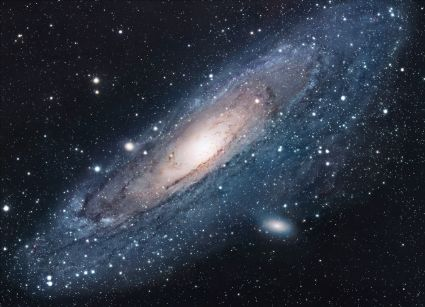
\includegraphics[height=4cm,width=4cm]{universe.jpg}
%         \caption{cite??}
%         \end{minipage}%
%         \begin{minipage}[t]{0.45\linewidth}
%         \centering
%         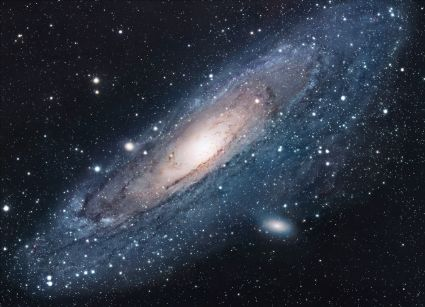
\includegraphics[heThis is the usage\cite{Wiki_bathtub,mankiw2014principles,finite} of Latex\cite{finite}.
	
% ight=4cm,width=4cm]{universe.jpg}
%         \caption{biao ti ?}
%         \end{minipage}
%     \end{figure}
%      %%% 需要的话,请在这里写图片说明,否则不要复制 %%%
    
% %% 合并图片(不要复制这句话)
%     \begin{figure}
%     \begin{minipage}{0.48\linewidth}
%       \centerline{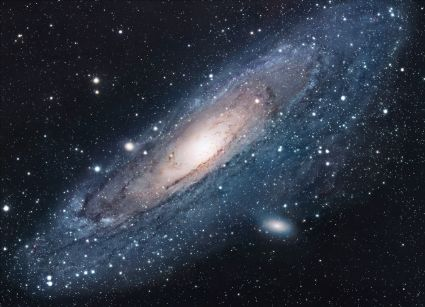
\includegraphics[width=4.0cm]{universe.jpg}}
%       \centerline{(a) Result 1}
%     \end{minipage}
%     \hfill
%     \begin{minipage}{.48\linewidth}
%       \centerline{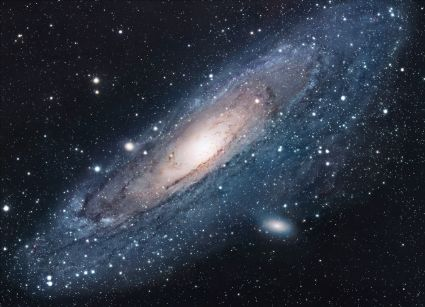
\includegraphics[width=4.0cm]{universe.jpg}}
%       \centerline{(b) Results 2}
%     \end{minipage}
%     %% 如果需要 多纵列的话
%     \vfill
%     \begin{minipage}{0.48\linewidth}
%       \centerline{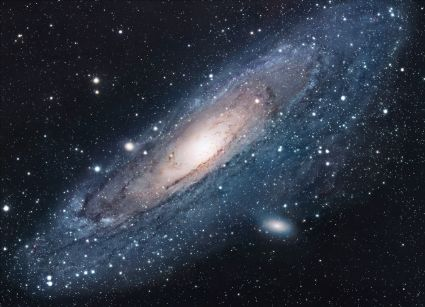
\includegraphics[width=4.0cm]{universe.jpg}}
%       \centerline{(c) Result 3}
%     \end{minipage}
%     \hfill
%     \begin{minipage}{0.48\linewidth}
%       \centerline{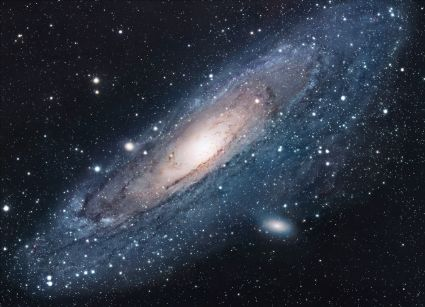
\includegraphics[width=4.0cm]{universe.jpg}}
%       \centerline{(d) Result 4}
%     \end{minipage}
%     %\end{tabular}
%     \caption{Examples of aaa}
%     \label{figures}
%     \end{figure}

%%%%%%%%%%%%%%%%%%%%%%%%%%%%%%%%%%%%%%%%%%%%%%%%%%%%%%%%%%%%%%%%%%%%%%%



\end{document}

%%
%% This work consists of these files mcmthesis.dtx,
%%                                   figures/ and
%%                                   code/,
%% and the derived files             mcmthesis.cls,
%%                                   mcmthesis-demo.tex,
%%                                   README,
%%                                   LICENSE,
%%                                   mcmthesis.pdf and
%%                                   mcmthesis-demo.pdf.
%%
%% End of file `mcmthesis-demo.tex'.
